\section{Anvendt rotårsaksanalyse}
Valget av rotårsaksanalyse rammeverk falt på prosessen beskrevet av Andersen og Fagerhaug på bakgrunn av tidligere arbeid med prosessen, fordi den er godt dokumentert og beskrevet, og passer til kriteriene for oppgaven. Prosessen innebærer syv steg (visualisert i figur \ref{fig:prosess}), der hvert steg anbefaler et sett verktøy for å fullføre det. Bruk av et eller flere verktøy kommer helt an på problemet som skal løses. Valg av verktøy i hver fase er basert på flytdiagrammene i kapittel 10 i boka av Andersen og Fagerhaug \cite{RCA}, som beskriver hvordan en velger riktig verktøy for oppgaven. Vi vurderte også hvilke verktøy som skal brukes selv, siden boken ikke er direkte tilpasset informasjonssikkerhetsoppgaver. Vi har også vurdert noen få verktøy utenfor det boken anbefaler. 

\begin{figure}[H]
    \centering
    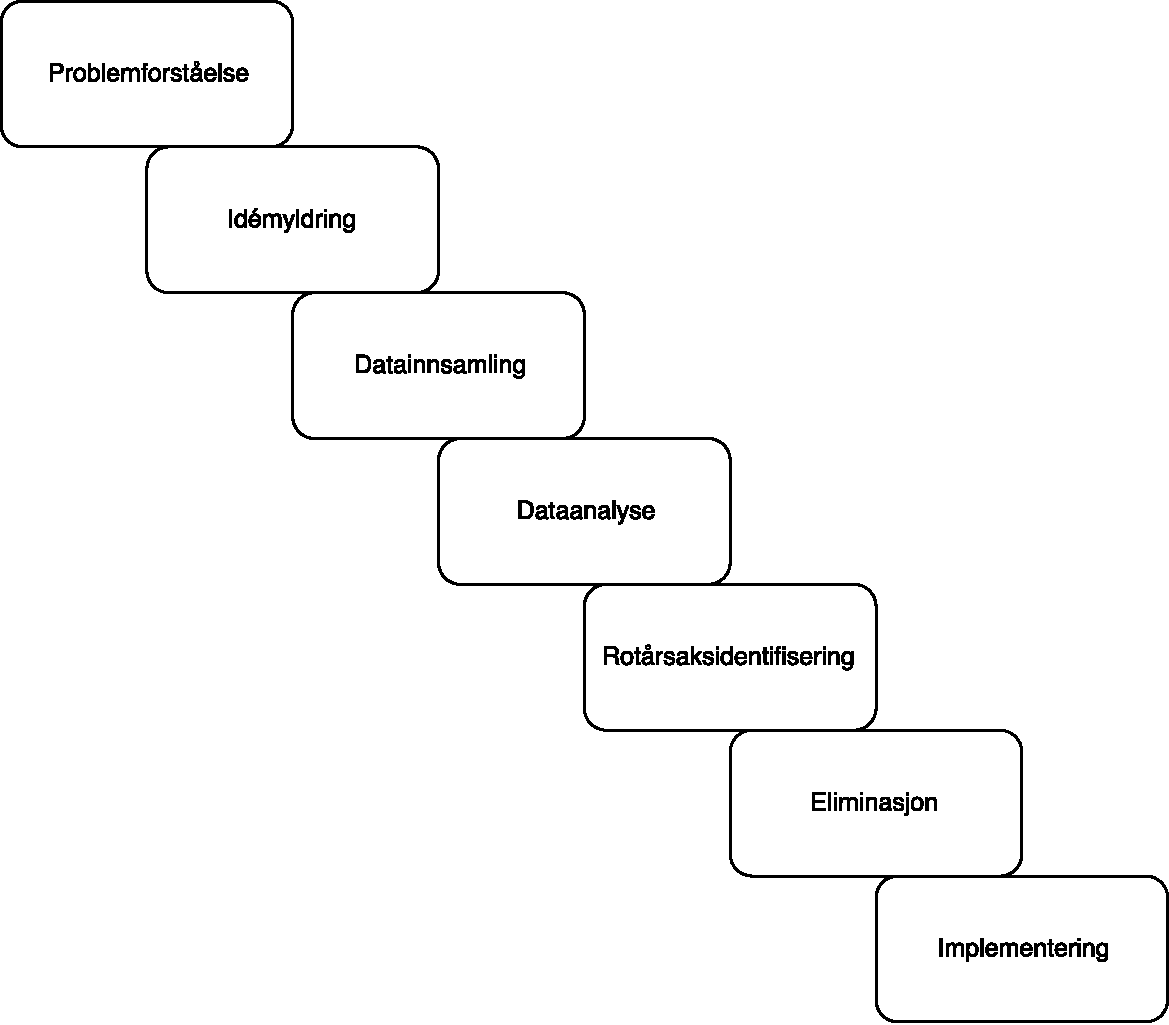
\includegraphics[scale=0.6]{prosess}
    \caption[RCA-prosess]{De syv fasene i rotårsaksanalyseprosessen}
    \label{fig:prosess}
\end{figure}

\subsection{Problemforståelse}
Problemforståelse går ut på å få en solid forståelse for problemet en ønsker å løse. Ofte er det ikke helt gitt at en forstår problemet fullt ut, men det er derimot kritisk at det gjøres. Det kan også hjelpe med å skape enighet rundt hva problemet omfatter, slik at alle er på samme side når analysen utføres. Det er også viktig for å passe på at ressursene som benyttes for analysen brukes effektivt videre. Under beskrives de verktøyene som ble brukt i analysen. 

\subsubsection{Flytdiagram}
Et flytdiagram viser flyten av aktiviteter i en prosess. Det kan være spesielt nyttig for å visualisere forretnings- og arbeidsprosesser. I informasjonssikkerhet kan det bli benyttet som en metode for å konkretisere og illustrere et problem ved- eller angrep mot virksomhetens aktiva. Formålet er å skape en detaljert forståelse for prosessen som har noe med problemet å gjøre \cite{RCA}.

\subsubsection{Kritiske hendelser}
Hovedpoenget med kritiske hendelser er å identifisere hva de mest kritiske symptomene i problemet er. Det kan hjelpe med å forstå hvilke aspekter ved problemet som trenger å løses, samt forstå problemets natur og konsekvenser for virksomheten \cite{RCA}. 

\subsection{Idémyldring}
Målet i denne fasen er å benytte ulike verktøy til å identifisere mulige rotårsaker, samt å skape enighet i saker hvor det er uenighet eller forskjellige synspunkter. Det eksisterer ofte på forhånd mistanker om hva rotårsaken kan være og det er viktig å ta i betraktning alle mulige årsaker, selv om de ved første øyekast kan virke irrelevante. Det er flere måter å strukturere idémyldringen på, men vi har benyttet oss av både muntlig og skriftlig idémyldring (også kjent som Idéskriving). Disse beskrives i nærmere detalj under. 

\subsubsection{Idémyldring}
Idémyldring er noe de fleste er kjent med fra tidligere. Målet er å generere så mange idéer som mulig om et gitt emne. I rotårsaksanalyse er målet stort sett å generere en liste over problemområder som kan forbedres, identifisere mulige konsekvenser, generere en liste over mulige årsaker til problemet og oppmuntre til å tenke på løsninger som kan eliminere problemet. Det finnes i hovedsak to typer idémyldring: strukturert og ustrukturert idémyldring. I strukturert idémyldring har hver deltaker sin tur med å komme med idéer. Dette fører til lik deltagelse og ingen som dominerer prosessen med egne idéer. I ustrukturert idémyldring kan hvem som helst komme med idéer når som helst. Dette er ofte mer spontant, men kan føre til at en person dominerer prosessen \cite{RCA}. 

\subsubsection{Idéskriving}
Idéskriving har samme hensikt som idémyldring, det eneste som skiller de to er måten det utføres på. Idéskriving utføres gjerne over nettet der en skriver ned idéer etterhvert som man kommer på de. Positive aspekter ved dette er at flere kan ha tilgang til prosessen, deltagerne kan beskrive mer detaljerte idéer, og det er også mulighet for å gjøre det anonymt dersom tema er sensitivt \cite{RCA}. 

\subsection{Datainnsamling}
I denne fasen er hovedoppgaven å samle inn så mye relevant informasjon om problemet som mulig. Ustrukturert og tilfeldig problemløsing har en tendens til å bli svært unøyaktig. Strukturert rotårsaksanalyse gir derimot et godt grunnlag for blant annet datainnsamlingen, som er en av de viktigste fasene i prosessen. Gjøres ikke denne grundig nok kan det få store konsekvenser for resultatene senere i oppgaven. Under beskrives verktøyene som ble brukt for å samle inn informasjon. 

\subsubsection{Spørreundersøkelser}
Spørreundersøkelser brukes når en er på utkikk etter å samle inn data om personers holdninger, følelser eller meninger om et spesifikt problem. En kan skille mellom to typer spørreundersøkelser: kvalitative og kvantitative spørreundersøkelser. Kvantitative undersøkelser handler om å få mange svar slik at en kan ta avgjørelser basert på tall som kan brukes til statistisk analyse. Kvalitative undersøkelser går ut på å samle detaljert informasjon om emnet. Dette kan hjelpe med blant annet å formulere hypoteser for å dirigere kvantitativ undersøkelse senere, eller å komplimentere en kvantitativ undersøkelse ved å bruke sitater fra åpne spørsmål \cite{KvalKvant}. 

\subsubsection{Intervjuer}
For intervjuer gjelder mye av det samme som ved spørreundersøkelser. Den store forskjellen er at det er direkte kontakt mellom intervjueren og intervjuobjektet. Intervjuer kan gjøres på forskjellige måter. En kan avtale et møte og intervjue øye til øye, eller det kan tas over telefon. Det er ofte høyere svarrespons og bedre kvalitet på svarene ettersom man er i mer kontakt. 

\subsection{Dataanalyse}
I denne fasen blir dataene fra forrige fase analysert og visualisert. Hovedmålet er å avklare mulige rotårsaker som har innvirkning på problemet, og hvilke av de som har størst innflytelse. Under beskrives de ulike verktøyene som ble brukt for å analysere dataene.

\subsubsection{Histogram}
Histogrammer, også kjent som søylediagram, brukes for å vise distribusjon og varians i et datasett. Dataene kan vises i form av lengde, tid, kostnad, mengde osv. Hovedoppgaven til et histogram er å presentere data på en oversiktlig måte slik at det er lett å se mulige relasjoner. I rotårsaksanalyse brukes det til å se hvilke årsaker som dominerer og for å forstå distribusjonen av forskjellige problemer, årsaker, konsekvenser osv. \cite{RCA} Det er viktig å ha minst 30 svar for å lage et gyldig histogram \cite{RCA}.

\subsubsection{Affinitetsdiagram}
Affinitetsdiagram er et verktøy som kan brukes til å analysere kvantitative data. Formålet er å gruppere data og finne underliggende relasjoner mellom de resterende gruppene. Dette medfører at en kan se relasjoner mellom tilsynelatende urelaterte data. I rotårsaksanalyse brukes det ofte til å utforske relasjoner mellom forskjellige årsaker, og gruppering av relaterte årsaker inn i klasser som kan analyseres kollektivt senere \cite{RCA}. 

\subsubsection{Statistisk analyse}
KOMMER!

\subsection{Rotårsaksidentifisering}
De foregående fasene har forhåpentligvis generert en liste over mulige rotårsaker og målet i denne er å identifisere de faktiske årsakene. Dette er ikke nødvendigvis så lett som det høres ut som. Noen ganger kreves det flere iterasjoner for å finne rotårsaken(e). Det finnes også mer avanserte verktøy enn de vi bruker her, men velger å styre unna for enkelhets skyld. Verktøy som ble brukt til identifisering er beskrevet under. 

\subsubsection{Årsak-virkningsdiagram (Fiskebeindiagram)}
Et typisk årsak-virkningsdiagram undersøker og analyserer relasjonen mellom et problem og dets årsaker. Det fungerer som en kombinasjon av idémyldring og systematisk analyse. Hovedformålet med verktøyet er å forstå hva som er årsaken til et gitt problem. Det brukes for å generere og gruppere årsaker, og evaluere årsakene til problemet for å finne ut hvilke som mest sannsynlig er rotårsaker. Det finnes to typer årsaks-virkningsdiagrammer: fiskebeindiagram og prosessdiagram. Et prosessdiagram er egentlig en samling av fiskebeindiagrammer der hver prosess har sitt eget diagram. Det finnes to ulike tilnærminger til å skape et fiskebeindiagram: spredningsanalyse og årsaksopplisting. Kort forklart, spredningsanalyse grupperer først og idémyldrer etterpå, mens årsaksopplisting idémyldrer først og grupperer etterpå \cite{RCA}. 

\subsection{Problemeliminering}
Denne fasen utgjør å planlegge mulige løsninger til problemet for å eliminere rotårsaken. Dette er en mer kreativ fase enn de foregående, siden løsninger varierer mye fra problem til problem. Boken til Fagerhaug og Andersen \cite{RCA} beskriver to mulige tilnærminger til denne fasen. En for å stimulere kreativitet når en leter etter løsninger, og to verktøy for å konstruere og utvikle løsninger. Vi har prøvd et verktøy fra hver tilnærming og de er beskrevet under. 

\subsubsection{De seks tenkehattene}
Formålet med de seks tenkehattene er å oppmuntre til å se på problemet og løsningene fra forskjellige synsvinkler. Det passer også på at idéene blir nøye kontrollert før beslutninger tas. Konseptet går ut på at personene får hver sin hatt som skal illustrere deres holdning til problemene \cite{RCA}. 

\begin{description}
    \item[Hvit hatt] skal være kald, nøytral og objektiv, personen skal fokusere på fakta.
    \item[Rød hatt] skal representere sinne, og skal bare fokusere på magefølelsen og egne følelser.
    \item[Svart hatt] skal være pessimistisk og negativ, og fokusere på hvorfor idéen er dårlig.
    \item[Gul hatt] er optimistisk og positiv, og skal fokusere på hvorfor idéen er bra og vil fungere.
    \item[Grønn hatt] representerer gresset, fruktbarhet og vekst, og skal fokusere på å vøre kreativ og komme på nye idéer.
    \item[Blå hatt] er koblet til himmelen, og skal fokusere på å se tingene fra et høyere perspektiv.
\end{description}

\subsubsection{Systematisk Innovativ Tenkning (SIT)}
SIT er basert på en såkalt ``lukket verden''. Dette betyr at løsningene på problemet ofte fokuseres i det fagområdet problemet eksisterer i. I rotårsaksanalyse brukes verktøyet til å finne kreative løsninger på problemer, og forsikre seg om at disse løsningene er brukbare og hører gjemme i fagfeltet. SIT baserer seg på å undersøke en eller flere kjernekomponenter ved hjelp av fem hovedprinsipper \cite{RCA}: 

\begin{description}
    \item[Attributtavhengighet] vurderer å endre en nøkkelvariabel i et produkt for å skape forbedring.
    \item[Komponentkontroll] ser på hvordan et produkt er knyttet til omgivelsene.
    \item[Erstatning] handler om å erstatte en del av et produkt med noe annet fra produktets omgivelser.
    \item[Forflytning] vurderer å forbedre problemet ved å fjerne en komponent. 
    \item[Oppdeling] har som må å splitte et produkts attributter i to, som for eksempel splittelsen av sjampo fra balsam.
\end{description}

\subsection{Løsningsimplementering}
I den siste fasen er målet å implementere løsningene som ble funnet i foregående fase. I vår rapport vil implementeringen beskrives til beste evne, men ikke implementeres siden vi ikke har mulighet til dette. Implementeringen inkluderer blant annet organisering, utvikling av en implementeringsplan, skape et konsensus om de nødvendige endringene og selvfølgelig implementeringen. Implementeringen av løsningen kan sies å være en suksess når symptomene forsvinner. Verktøyet vi valgte å benytte oss av i alle tre casene beskrives under. 

\subsubsection{Trediagram}
Et trediagram er et verktøy som er enkelt å bruke og er passende for å dele opp større oppgaver inn i mindre, mer håndterlige aktiviteter. Det er et verktøy som hjelper til å organisere arbeidet som må gjennomføres for å implementere tiltakene som er anbefalt. I rotårsaksanalyse benyttes dette for å strukturere oppgavene og planlegge implementeringsprosessen av løsningen. Et trediagram visualiserer hierarkiet i aktivitetene som må gjennomføres, eller enklere sagt, rekkefølgen ting må gjøres i for å fullføre implementeringen. 